  % kUML plain theme — override these styles in your preamble to restyle.
  \tikzset{
    kuml-class/.style={draw=black, fill=white, line width=0.6pt, rectangle, inner sep=0pt, font=\sffamily},
    kuml-interface/.style={kuml-class},
    kuml-enum/.style={kuml-class},
    kuml-stereotype/.style={font=\sffamily\itshape\small},
    kuml-classname/.style={font=\sffamily\bfseries},
    kuml-classname-abstract/.style={font=\sffamily\bfseries\itshape},
    kuml-feature/.style={font=\sffamily\footnotesize},
    kuml-association/.style={draw=black, line width=0.6pt, -{Stealth[length=2.2mm]}},
    kuml-generalization/.style={draw=black, line width=0.6pt, -{Triangle[length=3mm, open]}},
    kuml-realization/.style={draw=black, line width=0.6pt, dashed, -{Triangle[length=3mm, open]}},
    kuml-dependency/.style={draw=black, line width=0.5pt, dashed, -{Stealth[length=2mm]}},
    kuml-edge-plain/.style={draw=black, line width=0.6pt, -{Stealth[length=2.2mm]}},
    kuml-edge-bidi/.style={draw=black, line width=0.6pt, {Stealth[length=2.2mm]}-{Stealth[length=2.2mm]}},
    kuml-sysml2-edge-solid/.style={draw=black, line width=0.6pt, -{Stealth[length=2.2mm]}},
    kuml-sysml2-edge-dashed/.style={draw=black, line width=0.6pt, dashed, -{Stealth[length=2.2mm]}},
    kuml-sysml2-edge-dashed-noarrow/.style={draw=black, line width=0.6pt, dashed},
    kuml-sysml2-edge-binding/.style={draw=black, line width=0.6pt},
    kuml-sysml2-edge-generalization/.style={draw=black, line width=0.6pt, -{Triangle[length=3mm, open]}},
    kuml-sysml2-frame/.style={draw=black, line width=0.6pt, rectangle, inner sep=0pt, font=\sffamily},
    kuml-sysml2-edge-diamond-filled/.style={draw=black, line width=0.6pt, {Diamond[length=3mm]}-},
    kuml-sysml2-edge-diamond-open/.style={draw=black, line width=0.6pt, {Diamond[open, length=3mm]}-},
    kuml-sysml2-edge-containment/.style={draw=black, line width=0.6pt, {Circle[open, length=3mm]}-},
    kuml-c4-person/.style={draw=black, fill=white, line width=0.6pt, rectangle, rounded corners=16pt, inner sep=0pt, font=\sffamily},
    kuml-c4-system/.style={draw=black, fill=blue!10, line width=0.6pt, rectangle, inner sep=0pt, font=\sffamily},
    kuml-c4-container/.style={draw=black, fill=blue!20, line width=0.6pt, rectangle, inner sep=0pt, font=\sffamily},
    kuml-c4-component/.style={draw=black, fill=white, line width=0.6pt, rectangle, inner sep=0pt, font=\sffamily},
    kuml-c4-node/.style={draw=black, fill=white, line width=0.6pt, rectangle, dashed, inner sep=0pt, font=\sffamily},
    kuml-c4-code/.style={draw=black, fill=white, line width=0.6pt, rectangle, inner sep=0pt, font=\sffamily},
    kuml-c4-label/.style={font=\sffamily},
    kuml-c4-edge-label/.style={font=\sffamily\small},
    % ── BPMN styles ─────────────────────────────────────────────────────────
    kuml-bpmn-event/.style={circle,minimum size=28pt,draw=black,line width=1pt,font=\footnotesize,align=center,inner sep=2pt},
    kuml-bpmn-start/.style={kuml-bpmn-event,fill=white},
    kuml-bpmn-end/.style={kuml-bpmn-event,line width=3pt},
    kuml-bpmn-intermediate/.style={kuml-bpmn-event,double,double distance=2pt},
    kuml-bpmn-boundary/.style={kuml-bpmn-event,dashed},
    kuml-bpmn-gateway/.style={diamond,minimum size=36pt,draw=black,line width=1pt,aspect=1.4,font=\footnotesize,align=center,inner sep=0pt},
    kuml-bpmn-task/.style={rectangle,rounded corners=5pt,minimum width=80pt,minimum height=40pt,draw=black,line width=1pt,font=\footnotesize,align=center,text width=70pt,inner sep=4pt},
    kuml-bpmn-subprocess/.style={kuml-bpmn-task,double,double distance=2pt},
    kuml-bpmn-callactivity/.style={kuml-bpmn-task,line width=3pt},
    kuml-bpmn-pool/.style={rectangle,draw=black,line width=1.5pt,minimum width=200pt,minimum height=80pt,align=left},
    kuml-bpmn-pool-header/.style={rectangle,draw=black,line width=1pt,fill=gray!15,minimum width=25pt,font=\footnotesize\bfseries,align=center},
    kuml-bpmn-lane/.style={rectangle,draw=black,line width=0.7pt,fill=white,minimum width=175pt,minimum height=70pt,align=left},
    kuml-bpmn-lane-header/.style={rectangle,draw=black,line width=0.5pt,fill=gray!8,minimum width=20pt,font=\scriptsize,align=center},
    kuml-bpmn-flow/.style={->,>=stealth,draw=black,line width=0.8pt},
    kuml-bpmn-msgflow/.style={->,>=open triangle 45,draw=black,line width=0.8pt,dashed},
    kuml-bpmn-label/.style={font=\scriptsize,align=center},
    % ── Blueprint styles ────────────────────────────────────────────────────
    kuml-bp-band/.style={draw=none, rectangle, minimum height=2.0cm, font=\sffamily},
    kuml-bp-step/.style={draw, rounded corners=2pt, fill=white, minimum width=3.1cm, minimum height=1.4cm, align=center, font=\sffamily\small},
    kuml-bp-label/.style={font=\sffamily\bfseries, anchor=west},
    kuml-bp-phase/.style={font=\sffamily\bfseries, anchor=south},
    kuml-bp-line-interaction/.style={draw=blue!40!black, line width=0.8pt},
    kuml-bp-line-visibility/.style={draw=blue!40!black, line width=0.8pt, dashed},
    kuml-bp-line-internal/.style={draw=blue!40!black, line width=0.8pt, dotted},
    kuml-bp-line-label/.style={font=\sffamily\itshape\footnotesize, anchor=south east},
    kuml-bp-emotion/.style={draw=orange!80!black, line width=1pt, mark=*, mark size=2pt},
  }
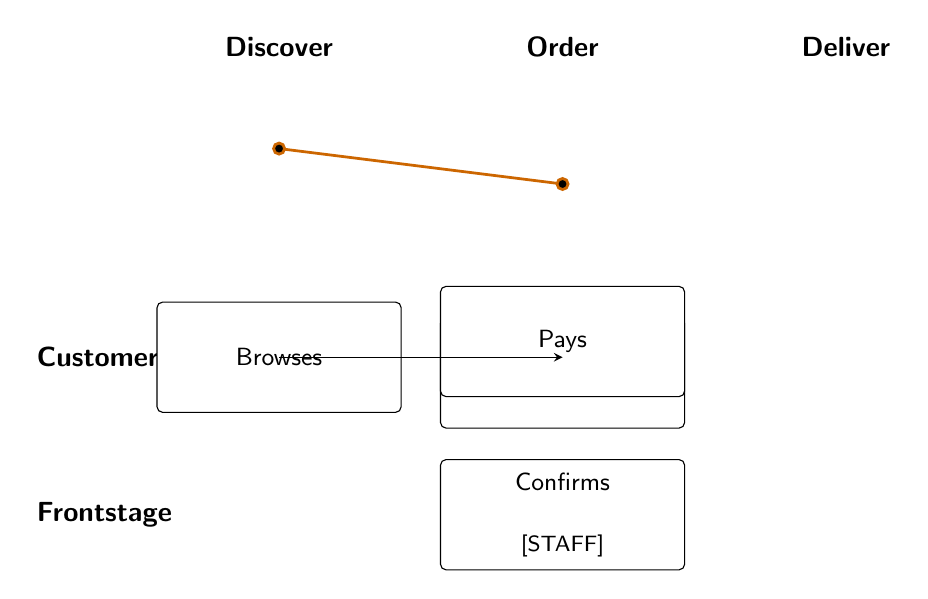
\begin{tikzpicture}[>=stealth]

  \node[kuml-bp-phase] at (1.80, 0.3) {Discover};
  \node[kuml-bp-phase] at (5.40, 0.3) {Order};
  \node[kuml-bp-phase] at (9, 0.3) {Deliver};

  \node[kuml-bp-label] at (-1.4, -3.40) {Customer Actions};
  \node[kuml-bp-label] at (-1.4, -5.40) {Frontstage};

  \draw[kuml-bp-emotion] plot coordinates {(1.80,-0.75) (5.40,-1.20)};

  \node[kuml-bp-step] at (1.80, -3.40) {Browses};
  \node[kuml-bp-step] at (5.40, -3.60) {Orders};
  \node[kuml-bp-step] at (5.40, -3.20) {Pays};
  \node[kuml-bp-step] at (5.40, -5.40) {Confirms\\\\{\footnotesize[STAFF]}};

  \draw[->] (1.80,-3.40) -- (5.40,-3.40);

\end{tikzpicture}
